\documentclass{beamer}
\setbeamertemplate{caption}[numbered]
\mode<presentation>{
	\usetheme{CambridgeUS}
	}
\usecolortheme{beaver}
\usepackage{graphicx}
\usepackage{multirow}

\title[Beamer Presentation]{Presentation on \textbf{Toward a Mobile Phone Based Solution for Microcredit in Rural Bangladesh}}
\author[1305031, 1305057]{Rukshar Alam(1305031) and Md.Saqib Hasan(1305057)}
\institute[BUET]{Bangladesh University of Engineering and Technology}

\begin{document}

\begin{frame}
\titlepage
\end{frame}

\begin{frame}
\frametitle{Outline of the presentation}
\tableofcontents
\end{frame}

\section{Introduction}
\begin{frame}

\begin{center}
{\LARGE \textbf{Introduction}}
\end{center}

\end{frame}

\begin{frame}
\frametitle{Microcredit?}
\begin{itemize}
\item What is \textbf{Microloan}?
\item Main functions of microcredit
\begin{itemize}
\item Provide the poor with a means to alleviate from poverty
\item Empower women
\end{itemize}
\end{itemize}
\end{frame}

\begin{frame}
\frametitle{History of Microcredit}
\begin{itemize}
\item Microcredit provided by institutions like Grameen Bank,BRAC
\item 250 Microfinance institutions globally, dealing with 154383.43 million USD
\item Dr. Muhammad Yunus and Grameen Bank awarded Nobel Prize in 2006
\end{itemize}
\end{frame}

\begin{frame}
\frametitle{Criticism}
\begin{itemize}
\item High Interest Rates
\item Failed Enterprenueships
\item Natural Disasters and Uncertainty
\item \textbf{Misuse of loan}
\end{itemize}
\end{frame}

\section{Background Study}

\begin{frame}
\begin{center}
{\LARGE \textbf{Background Study}}
\end{center}
\end{frame}

\begin{frame}
\begin{itemize}
\item Lots of Critical Analysis on Microcredit
\item Microcredit can change fate of the poor
\item Some serious situations leading to fates as worse as suicide
\item Mobile tech solutions to rural problems: Avaaj Uthalo
\item Tech solutions can solve problems such as rights issues,disease, human rights issues and cultural understanding
\end{itemize}
\end{frame}

\section{Statistics of the Jamalganj Upazila}

\begin{frame}

\begin{center}
{\LARGE \textbf{Statistics of the Jamalganj District}}
\end{center}

\end{frame}


\begin{frame}
\begin{figure}[h]
\centering
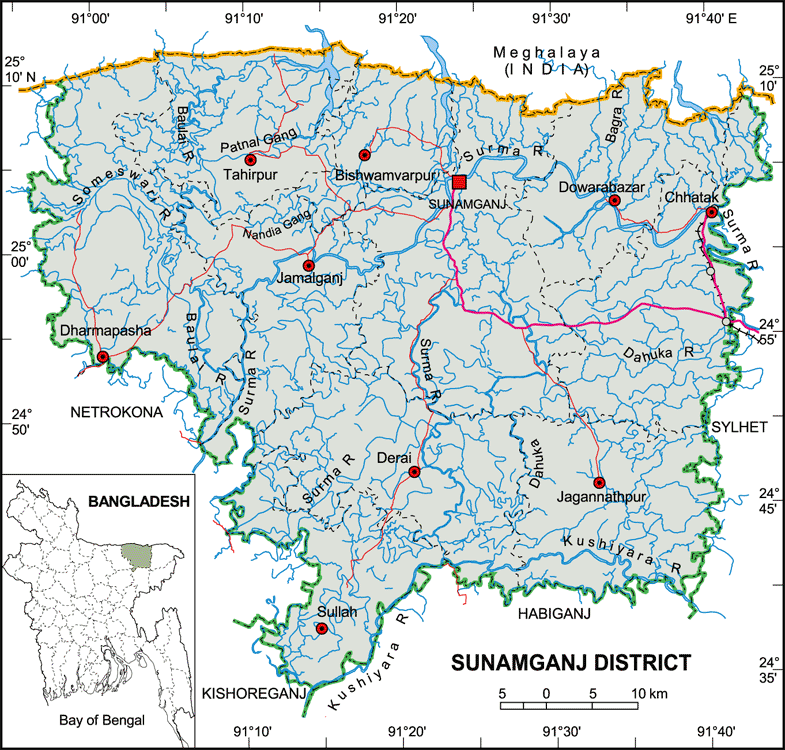
\includegraphics[width=0.6\textwidth]{map.png}
\caption{Map of Sunamganj}
\end{figure}
\end{frame}

\begin{frame}
\frametitle{Upazila Introduction and Literacy}
Located in Sunamganj District, Sylhet Division
\begin{figure}
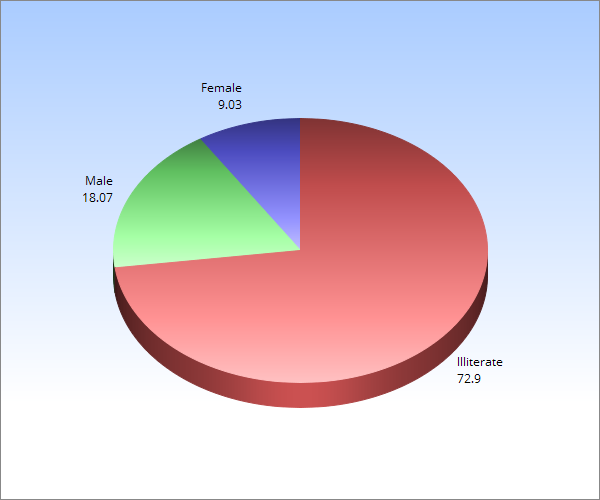
\includegraphics[width=0.6\textwidth]{g1.png}
\caption{Literacy Rate of Jamalganj.}
\end{figure}
\end{frame}

\begin{frame}
\frametitle{Main Occupations}
\begin{figure}[h]
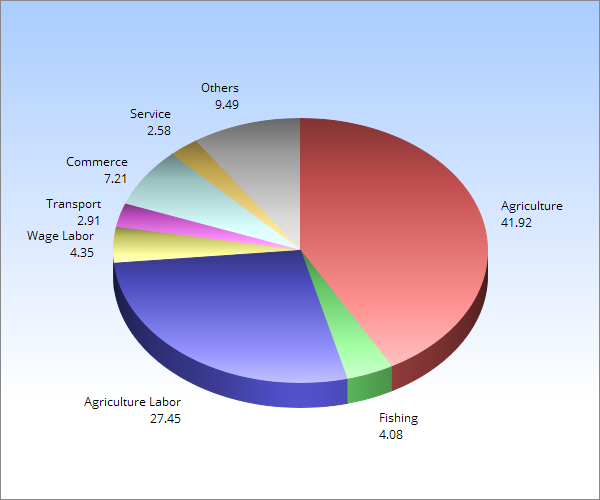
\includegraphics[width=0.6\textwidth]{g2.png}
\caption{Main Occupations of Jamalganj.}
\end{figure}
\end{frame}

\begin{frame}
\frametitle{Land Control}
\begin{figure}[h]
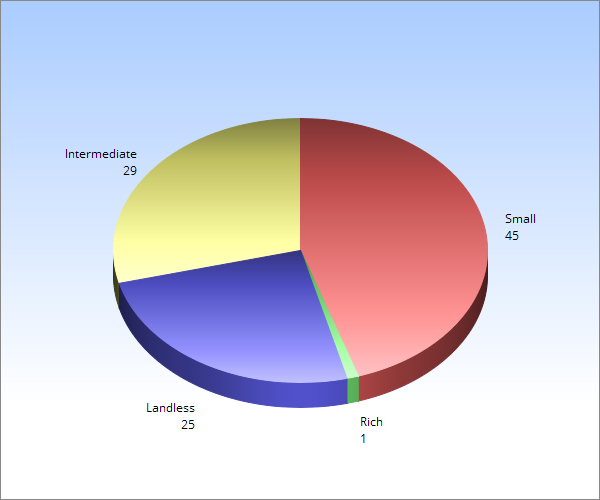
\includegraphics[width=0.6\textwidth]{g3.png}
\caption{Land Control in Jamalganj.}
\end{figure}

\end{frame}

\section{Case Studies}
\begin{frame}
\begin{center}
{\LARGE \textbf{Case Studies}}
\end{center}
\end{frame}

\begin{frame}
\frametitle{Data Collection}
Data collection on Microcredit transaction conducted in the Jamalganj Upazila in the division of Sylhet. Microcredit loans provided mainly to women of this region.
\end{frame}

\begin{frame}
\frametitle{Age Distribution}

\begin{table}[!h]
\centering
\begin{tabular}{|l|l|l|}
\hline
\textbf{Age Group} & \textbf{Number of Microcredit Clients} & \textbf{Percentage(\%)}\\
\hline
20-30 & 8 & 26.67\\
31-40 & 16 & 53.33\\
41-50 & 4 & 13.33\\
51 Above & 2 & 6.67\\
\hline
Total & 30 & 100\\
\hline
\end{tabular}
\caption{Age Distribution of Microcredit Client respondents}
\end{table}

\end{frame}

\begin{frame}
\frametitle{Educational Qualifications}

\begin{table}[!h]
\centering
\scalebox{0.9}{
\begin{tabular}{|l|l|l|}
\hline
\textbf{Education Qualification} & \textbf{Number of Microcredit Clients} & \textbf{Percentage(\%)}\\
\hline
No Formal Education & 6 & 20\\
Primary & 8 & 26.67\\
Middle & 10 & 33.33\\
S.S.C & 6 & 20\\
\hline
Total & 30 & 100\\
\hline

\end{tabular}
}
\caption{Educational Qualifications Distribution of Microcredit Client respondents}
\end{table}

\end{frame}

\begin{frame}
\frametitle{Family Member Distribution}

\begin{table}[!h]
\centering
\begin{tabular}{|l|l|l|}
\hline
\textbf{Family Member} & \textbf{Number of Microcredit Clients} & \textbf{Percentage(\%)}\\
\hline
1-2 & 1 & 3.33\\
3-5 & 15 & 50\\
6-8 & 13 & 43.34\\
9-11 & 1 & 3.33\\
\hline
Total & 30 & 100\\
\hline

\end{tabular}
\caption{Family Member Distribution of Microcredit Client respondents}
\end{table}

\end{frame}

\begin{frame}
\frametitle{Loan Distribution}

\begin{table}[!h]
\centering
\scalebox{0.9}{
\begin{tabular}{|l|l|l|}
\hline
\textbf{Amount of Loan} & \textbf{Number of Microcredit Clients} & \textbf{Percentage(\%)}\\
\hline
1000-5000 & 17 & 56.67\\
6000-10000 & 2 & 6.66\\
11000-15000 & 3 & 10\\
16000 Above & 8 & 26.67\\
\hline
Total & 30 & 100\\
\hline

\end{tabular}
}
\caption{Loan Distribution of Microcredit Client respondents}
\end{table}



\end{frame}

\begin{frame}
\frametitle{Demographics of Mobile User at Jamalganj}
\begin{figure}
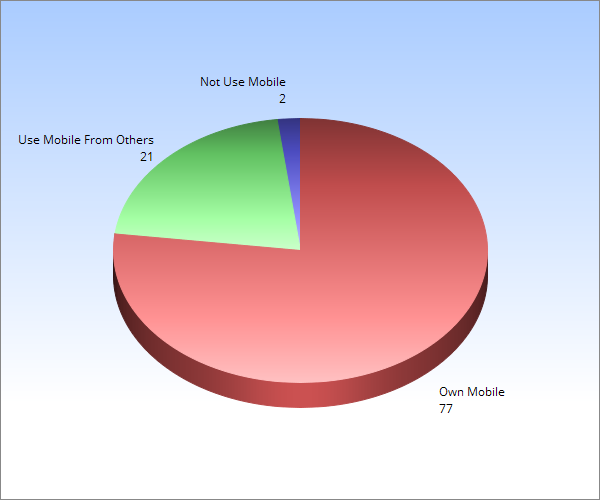
\includegraphics[width=0.6\textwidth]{g4.png}
\caption{Mobile user at Jamalganj in Sylhet.}
\end{figure}
\end{frame}

\begin{frame}
\frametitle{Comparative Study of People Involved in Microcredit}
\begin{figure}
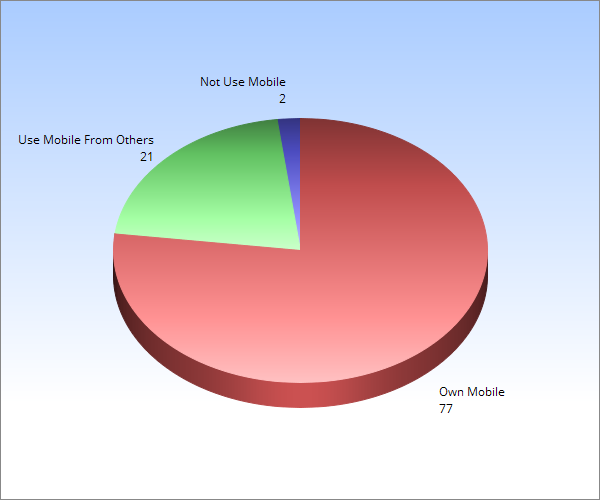
\includegraphics[width=0.6\textwidth]{g4.png}
\caption{Micro credit user at Jamalganj in Sylhet.}
\end{figure}
\end{frame}

\section{Some Problems of Microcredit}
\begin{frame}
\begin{center}
{\LARGE \textbf{Some Problems of Microcredit}}
\end{center}
\end{frame}

\begin{frame}
\frametitle{Categorizing the problems of Microcredit}
\begin{itemize}
\item Lack of Communication among Microcredit Organizations \pause
\item Inaccessible to the poorest \pause
\item Unbalance in the Microcredit System \pause
\item Mismanagement of Loan Money \pause
\item Extremely High Interest Rates \pause
\item Misuse of the \textbf{Women Empowerment} concept of Microcredit \pause
\end{itemize}
\end{frame}

\section{Proposed Solution}
\begin{frame}
\begin{center}
{\LARGE \textbf{Proposed Solution}}
\end{center}
\end{frame}

\begin{frame}


\begin{center}
A mobile based technology based on the concept of Short Message Service(SMS). User will create a mobile account and verfication for the loan will also be verified through the mobile account. All transactions will also be conducted through SMS using user's secret password. Designed to work on cheaper mobiles and uses Bangla font.
\end{center}

\end{frame}

\section{Advantages of the Proposed System}
\begin{frame}
\begin{center}
{\LARGE \textbf{Advantages of the Proposed System}}
\end{center}
\end{frame}

\begin{frame}
\frametitle{Categorizing the problems of Microcredit}
\begin{enumerate}
\item Proper Use of Money Can be Ensured \pause
\item Allocate Loans to the Poorest of the People \pause
\item Loans Must be Forwarded to the Client \pause
\item Risk Associated with Cash Money is Reduced \pause
\item Banks will Require Fewer Field Workers \pause
\end{enumerate}
\end{frame}

\section{Process}
\begin{frame}
\begin{center}
{\LARGE \textbf{Process}}
\end{center}
\end{frame}





\begin{frame}
\frametitle{Account Activation Requirements}
\begin{itemize}
\item Legitimate mobile account by government rules
\item Willingness
\end{itemize}
\end{frame}

\begin{frame}
\frametitle{Account Activation Process}
\begin{itemize}
\item Visit bank
\item Application form and documentation
\item Verification
\item Request sent and reply using mobile SMS
\item Unique password and required training
\end{itemize}
\end{frame}

\begin{frame}
\frametitle{Client Account Check}
\begin{itemize}
\item Entry of password
\item Request through mobile interface
\item Required information displayed
\end{itemize}
\end{frame}

\begin{frame}
\frametitle{Use of Loan Money}
\begin{itemize}
\item Nominated seller concept
\item Unique product code for each nominated seller's product
\item Client pursues transaction in the following steps:
\begin{itemize}
\item start service
\item select
\item enter code
\item get confirmation by SMS
\end{itemize}
\item Limitations of use of money
\item Live browsing
\end{itemize}
\end{frame}

\begin{frame}
\frametitle{Monthly Repayment}
\begin{itemize}
\item Reminder 5/7 days before due date
\item Travel to load point
\item Provide required info
\item Request sent to predefined number
\end{itemize}
\end{frame}

\begin{frame}
\frametitle{Reatailer's Sevices}
\begin{itemize}
\item Registration
\item Priviledges in case of cash money
\end{itemize}
\end{frame}

\begin{frame}
\frametitle{Issuing Loan}
\begin{itemize}
\item Go to bank
\item Documentation and verification
\item If yes,then:
\begin{enumerate}
\item terms and conditions
\item required training
\item mobile account to cash ratio (84:16)
\item finalize
\end{enumerate}
\item If no, then explain reason
\end{itemize}
\end{frame}



\section{Challenges of Proposed System}
\begin{frame}
\begin{center}
{\LARGE \textbf{Challenges of Proposed System}}
\end{center}
\end{frame}


\begin{frame}
\frametitle{List of Challenges}
\begin{itemize}
\item Lack of Education
\item Availability of Registered Shops
\item Implementation of a new concept
\end{itemize}
\end{frame}

\section{Conclusion}
\begin{frame}
\begin{center}
{\LARGE \textbf{Conclusion}}
\end{center}
\end{frame}


\begin{frame}
\frametitle{Concluding:}
\begin{center}
Data collection,analysis and a mobile tech solution to failing business endeavors of Microcredit system in rural Bangladesh.
\end{center}
\end{frame}




\begin{frame}
\begin{center}
{\LARGE \textbf{Thank You and Q/A}}
\end{center}
\end{frame}












\end{document}
\grid
